\documentclass[letterpaper,10pt,titlepage]{article}

\usepackage{graphicx}                                        
\usepackage{amssymb}                                         
\usepackage{amsmath}                                         
\usepackage{amsthm} 
\usepackage{verbatim}                                         

\usepackage{alltt}                                           
\usepackage{float}
\usepackage{color}
\usepackage{url}
\usepackage{fancybox}
\usepackage{verbatim}

\usepackage{balance}
\usepackage[TABBOTCAP, tight]{subfigure}
\usepackage{enumitem}
\usepackage{pstricks, pst-node}
\usepackage{texments}

\usepackage{geometry}
\geometry{textheight=9in, textwidth=6.5in}

\newcommand{\cred}[1]{{\color{red}#1}}
\newcommand{\cblue}[1]{{\color{blue}#1}}
\newcommand{\tab}{\hspace*{2em}}

\usepackage{hyperref}
\usepackage{geometry}

\def\name{Eric Timmerman, Stephanie Ison, Geoffrey Corey}

%% The following metadata will show up in the PDF properties
\hypersetup{
  colorlinks = true,
  urlcolor = black,
  pdfauthor = {\name},
  pdfkeywords = {cs325 ``algorithmic analysis''},
  pdftitle = {CS 325: Project 2},
  pdfsubject = {CS 325: Project 2},
  pdfpagemode = UseNone
}

\begin{document}
\hfill \name

\hfill \today

\hfill CS 325 Proj 2

\section{Run-time Analysis}

\subsection{Pseudo-code}
\subsubsection{Algorithm 1}
\begin{verbatim}
algorithm1 (num_list, num_list2):
    result = algorithm1_helper(num_list)
    result2 = algorithm1_helper(num_list2)
    total = result[0] - result2[0]
    return total


algorithm1_helper (num_list):
    min = sys.maxint
    total = 0
    for i in range(len(num_list) - 1, -1, -1):
        total = total + num_list[i]
        if (abs(total) < min):
            min = abs(total)
            left = i
            right = len(num_list)
    results = (min, left, right)
    return results
\end{verbatim}
\subsubsection{Algorithm 2}
\begin{verbatim}
algorithm2 (num_list, num_list2):
    num_list = algorithm2_helper (num_list)
    num_list2 = algorithm2_helper (num_list2)
    num_list.sort()
    num_list2.sort()
    min = num_list[0] - num_list2[0]
    return min

algorithm2_helper (num_list):
    list = []
    total = 0
    for i in range(len(num_list) - 1, -1, -1):
        total = total + num_list[i]
        list.append(total)
    return list
\end{verbatim}
\subsubsection{Algorithm 3}
\begin{verbatim}
algorithm3 (num_list):
    half = len(num_list)
    half = half / 2
    first_half = num_list[: half]
    second_half = num_list[half: ]
    min_left = algorithm34_helper(first_half)
    min_right = algorithm34_helper(second_half)
    second_half.reverse()
    algorithm1 (first_half, second_half)

algorithm34_helper(half):
    if len(half) <= 1:
        return 0
    left = half[ : len(half) / 2]
    right = half[len(half) / 2 : ]
    left_min = algorithm34_helper(left)
    right_min = algorithm34_helper(right)
    cross_min = min(right) + max(left)
    return min(left_min, right_min, cross_min)
\end{verbatim}
\subsubsection{Algorithm 4}
\begin{verbatim}
algorithm4 (num_list):
    half = len(num_list)
    half = half / 2
    first_half = num_list[: half]
    second_half = num_list[half: ]
    min_left = algorithm34_helper(first_half)
    min_right = algorithm34_helper(second_half)
    second_half.reverse()
    algorithm2 (first_half, second_half)
\end{verbatim}

\subsection{Asymptotic Analysis}
\subsubsection{Algorithm 1}
1 for loop ran twice n + n = 2n = O(n)
\subsubsection{Algorithm 2}
sort log n \\
sort log n = 2 log n = O (n + log n)
\subsubsection{Algorithm 3}
n log n x 2 = 2 O(n log n) + O(n)
\subsubsection{Algorithm 4}
O(n log n) + o(n)

\section{Proofs of Correctness}
\subsubsection{Algorithm 3}
\begin{verbatim}
If we assume that Algorithm 1 is correct. And assume that Algorithm 2 is not correct than for all values 

of x algorithm 1 y doesn't equal algorithm 2's y. 

Given Array1 [6, -7, -6] and Array2 [10, -2, 15]

Array1 sums [-7, -13, -6] Array2 sums [23, 13, 15]

Algorithm 1 would return -13 as the min of Array1 and find 13 of Array2 the Sum Closest to Zero = 0

Algorithm 2 would combine and sort the arrays into NewArray [-13, -7, -6, 13, 15, 23] then compares 

NewArray[0] + NewArray [Array1Size+1] which would return the Sum 0. Algorithm 1 and 2 have 

returned the same result which is a contradiction to the condition of Algorithm 2 being not correct thus 

it must be correct.
\end{verbatim}
\subsubsection{Algorithm 4}
\begin{verbatim}
Base Case: Array A of length = 1, that is the closest to zero value.

Inductive Hypothesis: For size array N the subarray of size k such that 0 < k < n is contained entirely in 

the first half, second half, or a combination of the suffix of the first half and a prefix of the second half. 

Inductive Step:

By the Inductive Hypothesis if array of size n+1 there will still be a subarray of size k such that k < n and 

k+1 is still less than or equal to n, which is still a subarray.
\end{verbatim}

\section{Experimental Analysis}
\verbatiminput{plotting.txt}
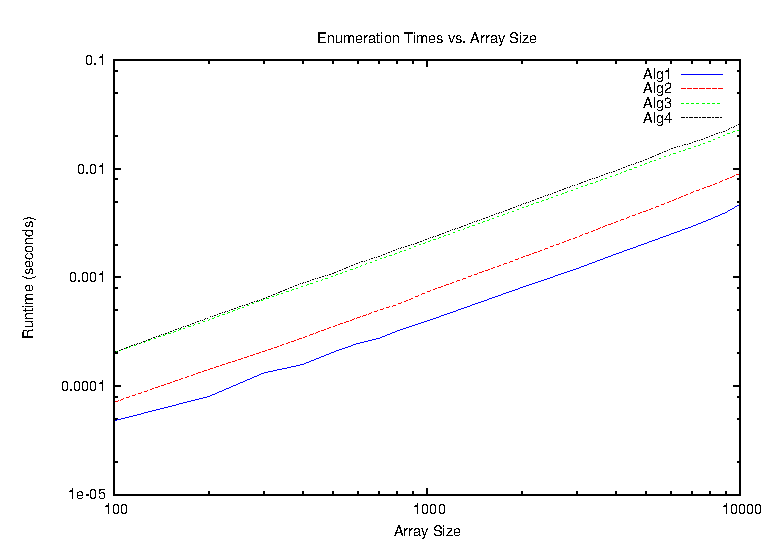
\includegraphics[width=\textwidth]{graph.eps}
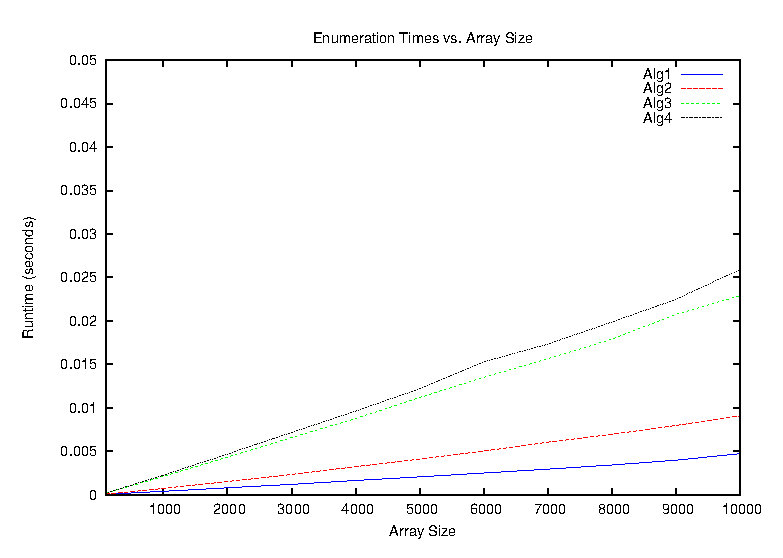
\includegraphics[width=\textwidth]{graph2.eps}

\section{Extrapolation and interpretation}

\subsection{Algorithms 3 and 4, largest dataset in 1 hour?}
\subsubsection{Algorithm 3}
Using 2 data points from the timing results in algorithm 3 (0.000204s, 100 and 0.022931s, 10000) and plugging them into the equation:
\begin{equation}\label{eq:Slope}
Slope = m = \frac{log(\frac{F_{1}}{F_{0}})}{log(\frac{x_{1}}{x_{0}})}
\end{equation}

resuls in $m = 1.0254$ as a log slope for the runtime of Algorithm 4. Using this value and the previous equation\eqref{eq:Slope}, we plug in 1 know data point (0.000204 seconds for an array of size 100) and the known time in 1 hour and solve for the array size.

\begin{equation*}
1.0254 = \frac{log(\frac{3600}{0.000204})}{log(\frac{x}{100})}
\end{equation*}
and we get that $x=1,167,260,000$.

*used \url{http://en.wikipedia.org/wiki/Log-log_plot} for help understanding log slope.
\subsubsection{Algorithm 4}
Using 2 data points from the timing results in algorithm 4 (0.000205s, 100 and 0.025944s, 10000) and plugging them into the equation:
\begin{equation}\label{eq:Slope}
Slope = m = \frac{log(\frac{F_{1}}{F_{0}})}{log(\frac{x_{1}}{x_{0}})}
\end{equation}

resuls in $m = 1.0254$ as a log slope for the runtime of Algorithm 4. Using this value and the previous equation\eqref{eq:Slope}, we plug in 1 know data point (0.000204 seconds for an array of size 100) and the known time in 1 hour and solve for the array size.

\begin{equation*}
1.04738 = \frac{log(\frac{3600}{0.000205})}{log(\frac{x}{100})}
\end{equation*}
and we get that $x=825,713,000$.

*used \url{http://en.wikipedia.org/wiki/Log-log_plot} for help understanding log slope.

\subsection{Experimental runtime and discrepancies}
\subsubsection{Algorithm 3}
Our asymptotic analysis said that algorithm 3 should be at least $O(n log n)$, but the runtime graph showed a graph that represented a more $C_{1}*n+C_{2}$ runtime. This could be due to how we implemented the algorithm as well as optimizations taken by the python interpreter. 
\subsubsection{Algorithm 4}
As with Algorithm 3, our asymptotic analysis said that Algorithm 4 should be dominated by by $O(n log n)$ but the runtime graph represented a more linear runtime ($C_{1}*n+C_{2}$). We very well could have done the algorithm incorrectly or the python interpreter could have introduced some optimizations that are unknown to us.


\end{document}
